\documentclass[11pt,letterpaper]{article}
\usepackage[lmargin=1in,rmargin=1in,tmargin=1in,bmargin=1in]{geometry}
\usepackage{../style/homework}
\setbool{quotetype}{true} % True: Side; False: Under
\setbool{hideans}{false} % Student: True; Instructor: False

% -------------------
% Content
% -------------------
\begin{document}

\homework{16: Due 04/10}{Mankind was born on Earth\dots it was never meant to die here.}{Joseph Cooper, Interstellar}

% Problem 1
\problem{10} Sketch the function $f(x)= (x + 6)^2 - 5$.
	\[
	\fbox{
	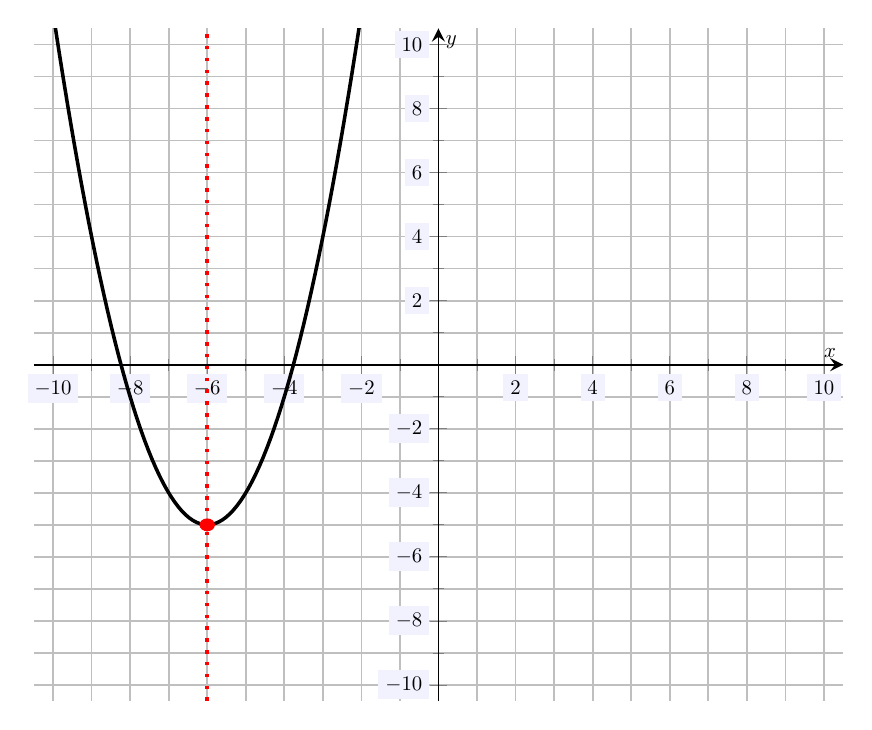
\begin{tikzpicture}[scale=1.5,every node/.style={scale=0.5}]
	\begin{axis}[
	grid=both,
	axis lines=middle,
	ticklabel style={fill=blue!5!white},
	xmin= -10.5, xmax=10.5,
	ymin= -10.5, ymax=10.5,
	xtick={-10,-8,-6,-4,-2,0,2,4,6,8,10},
	ytick={-10,-8,-6,-4,-2,0,2,4,6,8,10},
	minor tick = {-10,-9,...,10},
	xlabel=\(x\),ylabel=\(y\),
	]
	\draw[line width=0.03cm,red,dotted] (-6,-10.5) -- (-6,10.5);
	\addplot[line width=0.03cm,domain= -10.5:-1, samples=100] ({x},{(x + 6)^2 - 5});
	\draw[fill=red,draw=none] (-6,-5) circle (0.2);
	\end{axis}
	\end{tikzpicture}
	}
	\] \pspace

\sol Recall the vertex form of a quadratic function is $f(x)= a(x - P)^2 + Q$, where $(P, Q)$ is the vertex of the quadratic function and $a$ is the coefficient of $x^2$ from $f(x)= ax^2 + bx + c$. Observe that $f(x)= (x + 6)^2 - 5= 1 \big(x - (-6) \big)^2 + (-5)$. Therefore, $a= 1 > 0$ and $(P, Q)= (-6, -5)$. Therefore, the vertex is $(-6, -5)$ and the parabola opens downwards because $a= 1 > 0$. The axis of symmetry is $x= -6$. Therefore, the plot should be symmetric about this line. This gives the sketch given above. 



\newpage



% Problem 2
\problem{10} Find the equation of the quadratic function shown below. Be sure to fully justify why your answer is correct.
	\[
	\fbox{
	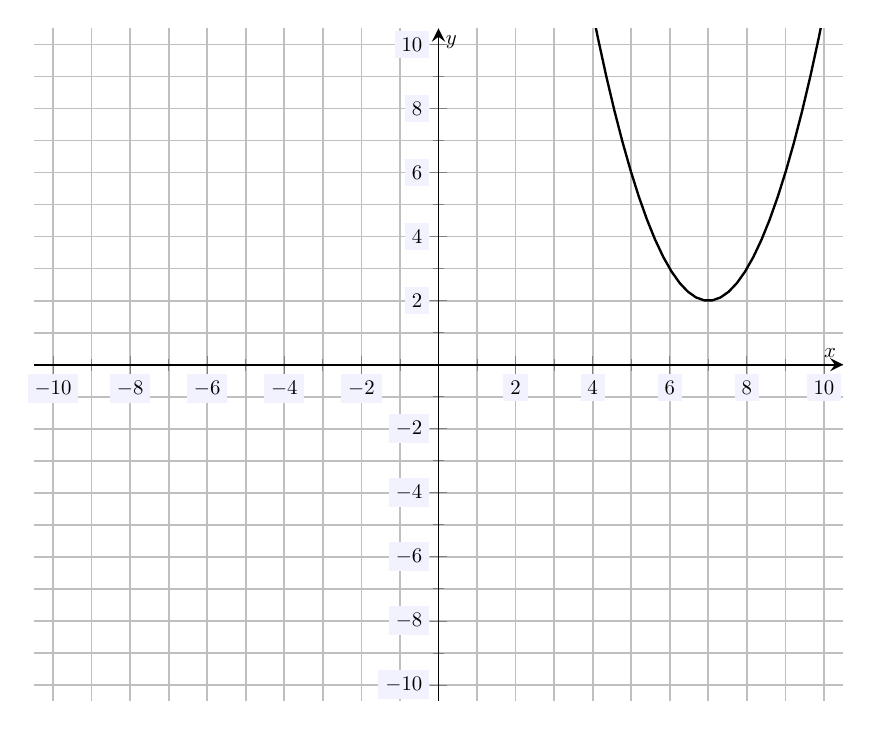
\begin{tikzpicture}[scale=1.5,every node/.style={scale=0.5}]
	\begin{axis}[
	grid=both,
	axis lines=middle,
	ticklabel style={fill=blue!5!white},
	xmin= -10.5, xmax=10.5,
	ymin= -10.5, ymax=10.5,
	xtick={-10,-8,-6,-4,-2,0,2,4,6,8,10},
	ytick={-10,-8,-6,-4,-2,0,2,4,6,8,10},
	minor tick = {-10,-9,...,10},
	xlabel=\(x\),ylabel=\(y\),
	]
	\addplot[line width= 0.02cm,samples=100,domain= -10.5:10.5] ({x},{(x - 7)^2 + 2});
	\end{axis}
	\end{tikzpicture}
	}
	\] \pspace

\sol Recall the vertex form of a quadratic function is $f(x)= a(x - P)^2 + Q$, where $(P, Q)$ is the vertex of the quadratic function and $a$ is the coefficient of $x^2$ from $f(x)= ax^2 + bx + c$. We know that if $a > 0$, then the quadratic function opens upwards and if $a < 0$, then it opens downwards. Clearly, because this parabola opens upwards, $a > 0$. Examining the plot, we can see that the vertex is $(P, Q)= (7, 2)$. Then we know that $f(x)= a(x - P)^2 + Q= a(x - 7)^2 + 2$. We can also see that the parabola contains the points $(5, 6)$ and $(9, 6)$. Then we know that when $x= 5$ that $y= 6$. But then\dots
	\[
	\begin{gathered}
	f(x)= a(x - 7)^2 + 2 \\
	f(5)= a(5 - 7)^2 + 2 \\
	6= a(-2)^2 + 2 \\
	6= 4a + 2 \\
	4= 4a \\
	a= 1
	\end{gathered}
	\] \pspace
Therefore, $f(x)= (x - 7)^2 + 2= x^2 - 14x + 51$. 



\newpage



% Problem 3
\problem{10} Consider the quadratic function $f(x)= -x^2 - 4x + 12$.
	\begin{enumerate}[(a)]
	\item Find $a, b, c$ for this quadratic function.
	\item Does $f(x)$ open upwards or downwards? Explain.
	\item Is this quadratic function convex or concave? Explain. 
	\item Find the minimum value of $f(x)$, if it exists. If it does not exist, explain why.  
	\item Find the maximum value of $f(x)$, if it exists. If it does not exist, explain why. 
	\end{enumerate} \pspace

\sol 
\begin{enumerate}[(a)]
\item A quadratic function has the form $ax^2 + bx + c$. But then we can see that for $f(x)$, $a= -1$, $b= -4$, and $c= 12$. \pspace

\item Because $a= -1 < 0$, this quadratic function opens downwards. \pspace

\item Because $a= -1 < 0$, this quadratic function is concave. \pspace

\item Because $a= -1 < 0$, this quadratic function has a no minimum value---the outputs of $f(x)$ get arbitrarily small. \pspace

\item Because $a= 1 > 0$, this quadratic function has a maximum value. We know the maximum value occurs at the vertex. So we need to find the vertex of $f(x)$. By completing the square, we have\dots
	\[
	\begin{gathered}
	-x^2 - 4x + 12 \\
	-(x^2 + 4x - 12) \\
	-\left(x^2 + 4x + \left(\frac{4}{2} \right)^2 - \left(\frac{4}{2} \right)^2 - 12 \right) \\
	-\left( (x^2 + 4x + 4) + (-4) - 12 \right) \\
	-\left( (x + 2)^2 - 16 \right) \\
	-(x + 2)^2 + 16
	\end{gathered}
	\]
Therefore, the vertex is $(-2, 16)$. But then the maximum value for $f(x)$ is 16 and occurs when $x= -2$. \pspace

Alternatively, using the `evaluation method', we know the vertex occurs when $x= -\frac{b}{2a}= -\frac{-4}{2(-1)}= -\dfrac{-4}{-2}= -2$. But then the $y$-coordinate of the vertex $f(-2)= -(-2)^2 - 4(-2) + 12= -4 + 8 + 12= 16$. Therefore, the vertex is $(-2, 16)$ and the maximum output of $f(x)$ is 16. 
\end{enumerate}



\newpage



% Problem 4
\problem{10} Consider the quadratic function $f(x)= (x + 3)^2 - 10$.
	\begin{enumerate}[(a)]
	\item Find $a, b, c$ for this quadratic function.
	\item Does $f(x)$ open upwards or downwards? Explain.
	\item Is this quadratic function convex or concave? Explain. 
	\item Find the minimum value of $f(x)$, if it exists. If it does not exist, explain why.  
	\item Find the maximum value of $f(x)$, if it exists. If it does not exist, explain why. 
	\end{enumerate} \pspace

\sol 
\begin{enumerate}[(a)]
\item A quadratic function has the form $ax^2 + bx + c$. But because $f(x)= (x + 3)^2 - 10= (x + 3)(x + 3) - 10= (x^2 + 6x + 9) - 10= x^2 + 6x - 1$, we can see that for $f(x)$, $a= 1$, $b= 6$, and $c= -1$. \pspace

\item Because $a= 1 > 0$, this quadratic function opens upwards. \pspace

\item Because $a= 1 > 0$, this quadratic function is convex. \pspace

\item Because $a= 1 > 0$, this quadratic function has a minimum value. We know the minimum value occurs at the vertex. So we need to find the vertex of $f(x)$. Recall the vertex form of a quadratic function is $f(x)= a(x - P)^2 + Q$, where $(P, Q)$ is the vertex of the quadratic function and $a$ is the coefficient of $x^2$ from $f(x)= ax^2 + bx + c$. Because $f(x)= (x + 3)^2 - 10= 1 \big(x - (-3) \big)^2 + (-10)$, we can see that $f(x)$ has vertex $(P, Q)= (-3, -10)$. But then the minimum value for $f(x)$ is $-10$ and occurs when $x= -3$. \pspace

\item Because $a= 1 > 0$, this quadratic function has no minimum value---the outputs of $f(x)$ get arbitrarily large. 
\end{enumerate}


\end{document}